\documentclass[11pt,a4paper]{article}
\usepackage{amsmath,amssymb}
\usepackage{booktabs}
\usepackage{array}
\usepackage{geometry}
\usepackage{pgfplots}
\pgfplotsset{compat=1.18}
\usepackage[hidelinks]{hyperref}
\geometry{margin=2.4cm}

% ---- source-level abbreviations only: every one of these prints as the longhand thesis symbol ----
\newcommand{\tq}{\tilde{q}}
\newcommand{\tD}{\tilde{D}}
\newcommand{\tF}{\tilde{F}}
\newcommand{\ttj}{\tilde{t}_{\rm j}}
\newcommand{\Euc}{{\rm Euc}}
\newcommand{\dec}{{\rm dec}}
\newcommand{\nr}{{\rm nr}}
\newcommand{\Flim}{F_{\rm lim}}
\newcommand{\tFlim}{\tilde{F}_{\rm lim}}
\newcommand{\Rint}{R_{\rm int}}
\newcommand{\Rdet}{R_{\rm det}}
\newcommand{\tcad}{t_{\rm cad}}
\newcommand{\tdec}{t_{\rm dec}}
\newcommand{\tj}{t_{\rm j}}
\newcommand{\Ravg}{\langle R_{\geq i}\rangle}
\newcommand{\Lmin}{L_{\rm min}}
\newcommand{\Lmax}{L_{\rm max}}
\newcommand{\Ldec}{L_{\rm dec}}
\newcommand{\Lj}{L_{\rm j}}
\newcommand{\Lnr}{L_{\rm nr}}
\newcommand{\Lnu}{L_\nu(t_{\rm dec})}

% ---- figure constants (thesis footnote-4 parameters, t_cad = 2 d; see Appendix B) ----
\pgfplotsset{
  /pgf/declare function={
    lgbase = -2.30103;   % log10(theta_j^2/2)
    xj     = 4.5;        % log10(L_j / L_dec)
    xnr    = 10.0933;    % log10(L_nr / L_dec)
    xtwo   = 5.1275;     % log10(L_2 / L_dec)     (i = 2)
    lqtwo  = 0.7366;     % log10(q_2^2)
    xten   = 6.8749;     % log10(L_10 / L_dec)    (i = 10)
    lqten  = 1.2009;     % log10(q_10^2)
    logRcad(\x,\xi,\lq) = lgbase + \lq + 1.5*(\x - \xi);
    logRtwo(\x)  = lgbase + 2*log10(1 + 10^((\x - xj)/3));
    logRthree(\x)= lgbase + 2*log10(1 + 10^((\x - xj)/5));
  }
}

\title{\textbf{Detection Rates of GRB Afterglows with a Luminosity Distribution}\\
\large An analytic derivation, continuing the bachelor's project and the project notes}
\author{}
\date{September 2026}

\begin{document}
\maketitle
\thispagestyle{empty}

\section*{Summary}

The bachelor's project (``Detection Rates of Gamma-Ray Burst Afterglows in Optical Surveys: An Analytic Approach'', referred to below as \emph{the thesis}) and the project notes derive the rate $R_{\geq i}$ at which a survey with limiting flux $\Flim$ and cadence $\tcad$ detects afterglows at least $i$ times, under the assumption that \emph{all afterglows are identical} and only their distance $D$ and viewing angle $\theta_{\rm obs}$ vary. Here we relax that assumption in the simplest possible way: the afterglows keep a common light-curve \emph{shape}, but their \emph{luminosity} is drawn from a power-law distribution. We

\begin{enumerate}
\item summarise the single-luminosity results that are needed (Section~\ref{sec:previous}),
\item introduce the luminosity distribution and work out how every quantity of the model scales with luminosity (Section~\ref{sec:lf}),
\item write the full detection-rate integral (Section~\ref{sec:integral}),
\item solve it analytically, case by case (Section~\ref{sec:solution}), and
\item read off the detected-luminosity distribution and collect the final results (Sections~\ref{sec:detected}--\ref{sec:summary}).
\end{enumerate}

The main outcome is that the detection rate of a population is \emph{not} the single-luminosity rate at some typical luminosity: the rate of a single burst rises as $L^{3/2}$ until its detection horizon hits a wall (the cadence horizon reaching the edge of the Euclidean volume, or the whole beaming cone becoming visible), and saturates beyond it. Integrated over a power law $\propto L^{\alpha}$, this produces three regimes -- dominated by the faint end, by the ``knee'' luminosity at the wall, or by the bright end -- with different scalings of the rate with $\Flim$ and $\tcad$ than in the single-luminosity model.

\section*{Notation}

All symbols are those of the thesis (equation numbers in square brackets refer to it). Only five new symbols are introduced, all in Section~\ref{sec:lf}: the luminosity $L$, its distribution $\phi(L)$ with index $\alpha$ and bounds $\Lmin,\Lmax$, and the threshold luminosities $\Ldec,\Lj,\Lnr,L_i$.

\begin{center}\footnotesize
\renewcommand{\arraystretch}{1.2}
\begin{tabular}{@{}l p{8.3cm}@{}}
\toprule
$q\equiv\theta_{\rm obs}/\theta_j$,\; $\tq\equiv q-1$ & normalised viewing angle; $\theta_j$ = jet half-opening angle \\
$q_\dec = 1+(\Gamma_0\theta_j)^{-1}$,\; $q_{\rm j}=2$,\; $q_\nr=\sqrt2/\theta_j$ & angles at which the off-axis light curve joins the on-axis one at $\tdec$ and at $\tj$; $q_\nr$ corresponds to $\theta_{\rm obs}=\sqrt2$ [29--31]\\
$\tdec$,\; $\tj=\tdec(\Gamma_0\theta_j)^{8/3}$,\; $\ttj\equiv\tj/\tdec$ & deceleration time, jet-break time; note $\tq_\dec=\ttj^{-3/8}$ \\
$\tF_\nu(t)\equiv F_\nu(t)/F_\nu(\tdec)$ & normalised on-axis light curve (PLS~G) [21] \\
$t_p(q)$,\; $\tF_p(q)\equiv F_p(q)/F_\nu(\tdec)$ & peak time and normalised peak flux of an off-axis observer [32, 33] \\
$D$,\; $D_\Euc$,\; $\tD\equiv D/D_\Euc$ & distance; radius of the Euclidean volume; normalised distance \\
$\mathcal R$,\; $\Rint=\tfrac43\pi\mathcal R D_\Euc^3$ & GRB rate density; total GRB rate inside $D_\Euc$ [35, 36] \\
$\Flim$,\; $\tFlim\equiv\Flim/F_\nu(\tdec,D_\Euc)$ & limiting flux of the survey; normalised limiting flux [38] \\
$D_{\max}(q)$,\; $q_\Euc$ & maximal detectable distance at angle $q$; angle at which $D_{\max}=D_\Euc$ [38, 40] \\
$\tcad$,\; $i$,\; $\tau_{\rm det}$,\; $P_{\geq i}$ & cadence; required number of detections; $\Delta t_{\rm det}/\tcad$; probability of $\geq i$ detections [54, 60] \\
$D_i$,\; $q_i$ & distance at which $\tau_{\rm det}=i$; angle at which $D_{\max}(q_i)=D_i$ [63, 64] \\
$\Rdet$,\; $R_{\geq i}$,\; $R(q,D)\equiv\tfrac12\theta_j^2q^2\tD^3\Rint$ & detection rates; rate contributed by the box $[0,q]\times[0,D]$ (thesis p.~24)\\
\midrule
$L\equiv\Lnu$ & on-axis spectral luminosity of a burst at $\tdec$ -- the normalisation of [34] \\
$\phi(L)\propto L^{\alpha}$ on $[\Lmin,\Lmax]$ & luminosity distribution (a probability density in $L$) \\
$\Ldec,\ \Lj,\ \Lnr,\ L_i$ & luminosities at which $q_\Euc(L)=q_\dec,\ q_{\rm j},\ q_\nr,\ q_i$ \\
$\Ravg$ & detection rate averaged over the luminosity distribution \\
\bottomrule
\end{tabular}
\end{center}

\noindent The index of the luminosity distribution is called $\alpha$ as is customary for GRB luminosity functions; it is the only $\alpha$ in this document (the temporal decay indices of thesis Table~2 are always written out as $-3(p-1)/4$ and $-p$). The detection count is called $i$ throughout, following the later sections of the project notes (the thesis uses $k$); consequently $i$ is never used as a generic index here.

\section{Summary of the single-luminosity results}
\label{sec:previous}

\subsection{Population, light curve and the detection integral}

The population model of thesis \S3.1 is: a spherical Euclidean universe of radius $D_\Euc$; GRBs distributed uniformly in volume with rate density $\mathcal R$ and uniformly in $\cos\theta_{\rm obs}$; and \emph{identical internal parameters} for all afterglows, so that the only free parameters of an event are $D$ and $\theta_{\rm obs}$. The total GRB rate inside the volume is
\begin{equation}
\Rint=\mathcal R\int_{V_\Euc}dV=\frac43\pi\mathcal R D_\Euc^3 . \tag{thesis 36}
\end{equation}

An observer at $q=\theta_{\rm obs}/\theta_j$ sees the on-axis light curve only from the joining time $t_p(q)$ onwards,
\begin{equation}
t_p(q)=\begin{cases}\tdec, & q<q_\dec,\\ \tj\,\tq^{8/3}, & q_\dec<q<q_{\rm j}\ \text{(phase II)},\\ \tj\,\tq^{2}, & q_{\rm j}<q<q_\nr\ \text{(phase III)},\end{cases}
\tag{thesis 32}
\end{equation}
so the peak flux received is the on-axis flux at that time, $F_p(q)=F_\nu(t_p(q))$. With the PLS~G on-axis light curve normalised at $\tdec$,
\begin{equation}
\tF_\nu(t)\equiv\frac{F_\nu(t)}{F_\nu(\tdec)}=\begin{cases}(t/\tdec)^{-3(p-1)/4}, & \tdec<t<\tj\ \text{(phase II)},\\[2pt] \ttj^{-3(p-1)/4}\,(t/\tj)^{-p}, & \tj<t<t_\nr\ \text{(phase III)},\end{cases}
\tag{thesis 21}
\end{equation}
the normalised peak flux becomes
\begin{equation}
\label{eq:Fp}
\tF_p(q)\equiv\frac{F_p(q)}{F_\nu(\tdec)}=\tF_\nu\bigl(t_p(q)\bigr)=
\begin{cases}1, & q<q_\dec,\\[2pt] (\tq/\tq_\dec)^{-2(p-1)}=\ttj^{-3(p-1)/4}\,\tq^{-2(p-1)}, & q_\dec<q<q_{\rm j},\\[2pt] \tq_\dec^{-2}\,(\tq/\tq_\dec)^{-2p}=\ttj^{-3(p-1)/4}\,\tq^{-2p}, & q_{\rm j}<q<q_\nr,\end{cases}
\tag{thesis 33}
\end{equation}
where the two forms on each line are equal because $\tq_\dec=\ttj^{-3/8}$. $\tF_p(q)$ is a decreasing function of $q$: the further off-axis, the later the light curve is joined and the fainter its peak.

The flux received from a burst at distance $D$ and angle $q$ is then
\begin{equation}
F_p(q,D)=\frac{\Lnu\,\tF_p(q)}{4\pi D^2},
\tag{thesis 34}
\end{equation}
where $\Lnu=4\pi D^2F_\nu(\tdec,D)$ is the on-axis spectral luminosity at the deceleration time; it is this single number that fixes the brightness of the whole (identical) population, and it is the quantity we will later distribute. A survey detects the burst if $F_p(q,D)>\Flim$, so the detection rate is
\begin{equation}
\Rdet=4\pi\theta_j^2\mathcal R\int_0^{q_\nr}dq\,q\int_0^{D_\Euc}dD\,D^2\;\Theta\bigl(F_p(q,D)-\Flim\bigr),
\tag{thesis 37}
\end{equation}
where the small-angle approximation $d\cos\theta_{\rm obs}\approx\theta_j^2\,q\,dq$ was used, and $q_\nr=\sqrt2/\theta_j$ is defined so that $\tfrac12\theta_j^2q_\nr^2=1$ exactly (the beaming factor $f_b=\theta_j^2/2$ is thus built in: $\Rdet\to\Rint$ when everything is detected). The distance out to which a burst at angle $q$ can be seen follows from $F_p(q,D_{\max})=\Flim$,
\begin{equation}
\tD_{\max}(q)\equiv\frac{D_{\max}(q)}{D_\Euc}=\tFlim^{-1/2}\,\tF_p(q)^{1/2},\qquad
\tFlim\equiv\frac{\Flim}{F_\nu(\tdec,D_\Euc)}=\frac{4\pi D_\Euc^2\,\Flim}{\Lnu},
\tag{thesis 38}
\end{equation}
and performing the $D$ integral in [37] gives
\begin{equation}
\Rdet=\theta_j^2\Rint\int_0^{q_\nr}dq\,q\,\min\bigl(\tD_{\max}^3(q),\,1\bigr).
\tag{thesis 39}
\end{equation}
The $\min$ expresses the two possible walls of the detection region: the flux horizon $D_{\max}(q)$ or the edge of the volume $D_\Euc$.

\subsection{The Euclidean angle $q_\Euc$ and the most-contributing point}

The angle at which the flux horizon reaches the edge of the volume, $D_{\max}(q_\Euc)=D_\Euc$, i.e. $\tF_p(q_\Euc)=\tFlim$, is
\begin{equation}
\tq_\Euc=\begin{cases}(\Gamma_0\theta_j)^{-1}\,\tFlim^{-1/(2(p-1))}, & q_\dec<q_\Euc<q_{\rm j},\\[2pt] (\Gamma_0\theta_j)^{-(p-1)/p}\,\tFlim^{-1/(2p)}, & q_{\rm j}<q_\Euc<q_\nr .\end{cases}
\tag{thesis 40}
\end{equation}
For angles $q<q_\Euc$ every burst inside the volume is detected; for $q>q_\Euc$ only those closer than $D_{\max}(q)<D_\Euc$. The limiting fluxes at which $q_\Euc$ coincides with the three special angles separate the four ranges of the thesis,
\begin{equation}
\label{eq:Flimx}
\tF_{\rm lim,dec}=\tF_p(q_\dec)=1,\qquad
\tF_{\rm lim,j}=\tF_p(q_{\rm j})=\tq_\dec^{\,2(p-1)},\qquad
\tF_{\rm lim,nr}=\tF_p(q_\nr)=\tq_\dec^{-2}\bigl(\tq_\nr/\tq_\dec\bigr)^{-2p},
\tag{thesis 45}
\end{equation}
range~I being $\tFlim>1$ (even an on-axis burst at $D_\Euc$ is too faint), range~II $\tF_{\rm lim,j}<\tFlim<1$, range~III $\tF_{\rm lim,nr}<\tFlim<\tF_{\rm lim,j}$, and range~IV $\tFlim<\tF_{\rm lim,nr}$ (everything is detected).\footnote{Thesis Eq.~45 as printed shows $\tF_{\rm lim,j}=\tq_\dec^{-2(p-1)}$; the positive exponent is the one consistent with Eq.~[33] and with the value $10^{-4.5}$ quoted in thesis Fig.~11 for $\tq_\dec=10^{-1.5}$, $p=2.5$.}

The exact integral [39] is elementary but cumbersome (thesis Eqs.~41--44). The thesis instead uses the density of detected events per logarithmic interval,
\begin{equation}
\frac{d\Rdet}{d\log D\,d\log q}=4\pi\theta_j^2\mathcal R\,q^2D^3=6\Rint\Bigl(\frac{q}{q_\nr}\Bigr)^2\tD^3,
\tag{thesis 46}
\end{equation}
to locate the \emph{most contributing point}: along the flux horizon $D_{\max}(q)\propto\tq^{-(p-1)}$ or $\tq^{-p}$ falls faster than $q^{-2/3}$, so $q^2D_{\max}^3(q)$ decreases with $q$ and the detections are dominated by the smallest angle on the horizon, i.e. by the corner where $D_{\max}(q)$ meets whatever caps the distance ($D_\Euc$ here; the cadence distance $D_i$ below). The rate is then approximated by the rate of the box $[0,q_\star]\times[0,D_\star]$ below and to the left of that corner,
\begin{equation}
\label{eq:RqD}
R(q,D)\equiv\theta_j^2\Rint\int_0^{q}dq'\,q'\,\tD^3=\tfrac12\,\theta_j^2\,q^2\,\tD^3\,\Rint ,
\end{equation}
evaluated at $(q_\star,D_\star)$ (thesis p.~24; project notes Eq.~29). This gives thesis Eq.~52,
\begin{equation}
\label{eq:Rdet52}
\Rdet\approx\tfrac12\theta_j^2\Rint\begin{cases}
q_\dec^2\,\tFlim^{-3/2}, & 1<\tFlim\ \text{(range I)},\\[3pt]
q_\Euc^2=\Bigl((\Gamma_0\theta_j)^{-1}\tFlim^{-1/(2(p-1))}+1\Bigr)^2, & \tF_{\rm lim,j}<\tFlim<1\ \text{(range II)},\\[3pt]
q_\Euc^2=\Bigl((\Gamma_0\theta_j)^{-(p-1)/p}\tFlim^{-1/(2p)}+1\Bigr)^2, & \tF_{\rm lim,nr}<\tFlim<\tF_{\rm lim,j}\ \text{(range III)},\\[3pt]
q_\nr^2=2\theta_j^{-2}, & \tFlim<\tF_{\rm lim,nr}\ \text{(range IV)},
\end{cases}
\tag{thesis 52}
\end{equation}
The corners are $(q_\dec,D_\dec)$ in range~I, with the on-axis horizon $\tD_\dec=\tFlim^{-1/2}$; $(q_\Euc,D_\Euc)$ in ranges~II and III; and $(q_\nr,D_\Euc)$ in range~IV, where everything is detected. Thesis Fig.~11 shows that this approximation reproduces the exact integral to within a factor of order unity everywhere (the worst case being a factor 4 near $\tF_{\rm lim,j}$).

\subsection{Cadence: the rate of $\geq i$ detections}
\label{sec:cadence}

A survey observes the same field every $\tcad$. The number of detections of an event is set by the ratio of the time it stays above the limiting flux to the cadence,
\begin{equation}
\tau_{\rm det}\equiv\frac{\Delta t_{\rm det}}{\tcad}\approx\frac{t_+(D)}{\tcad},\qquad F_\nu(t_+,D)=\Flim\ \Longleftrightarrow\ \tF_\nu(t_+)=\tD^2\,\tFlim,
\tag{thesis 54, 55}
\end{equation}
where $t_+$ is the time at which the on-axis light curve at distance $D$ fades below $\Flim$ (the approximation $\Delta t_{\rm det}\approx t_+$ drops the joining time $t_-\approx t_p(q)$). The probability of at least $i$ detections is
\begin{equation}
P_{\geq i}(\tau_{\rm det})=\begin{cases}0, & \tau_{\rm det}<i-1,\\ \tau_{\rm det}-(i-1), & i-1\le\tau_{\rm det}<i,\\ 1, & i\le\tau_{\rm det},\end{cases}
\tag{thesis 60}
\end{equation}
and the rate of events detected at least $i$ times is
\begin{equation}
R_{\geq i}=4\pi\theta_j^2\mathcal R\int_0^{q_\nr}dq\,q\int_0^{D_\Euc}dD\,D^2\;\Theta\bigl(F_p(q,D)-\Flim\bigr)\,P_{\geq i}\bigl(\tau_{\rm det}(D)\bigr).
\tag{thesis 58}
\end{equation}
(The factor $\Theta(F_p-\Flim)$ is implicit in the thesis through $\Delta t_{\rm det}>0$; it is written out here because the approximation $\Delta t_{\rm det}\approx t_+$ no longer enforces it.) For $i\geq2$ the thesis (\S3.2.3) replaces the ramp by a step, $P_{\geq i}\approx\Theta(\tau_{\rm det}-i)$, because the contribution of the ramp is dominated by its upper end; this is accurate to a few per cent. The step selects $D<D_i$, where $D_i$ is the distance at which the on-axis light curve stays above the limit for exactly $i$ cadences, $t_+(D_i)=i\,\tcad$:
\begin{equation}
\label{eq:Di}
\tD_i^{\,2}=\frac{\tF_\nu(i\,\tcad)}{\tFlim}
\qquad\Longrightarrow\qquad
\tD_i=\tFlim^{-1/2}\begin{cases}(i\,\tcad/\tdec)^{-3(p-1)/8}, & i\,\tcad<\tj,\\[2pt] \ttj^{-3(p-1)/8}\,(i\,\tcad/\tj)^{-p/2}, & i\,\tcad>\tj .\end{cases}
\tag{thesis 63}
\end{equation}
The corresponding angle $q_i$ is where the flux horizon meets this cap, $D_{\max}(q_i)=D_i$, i.e. $\tF_p(q_i)=\tF_\nu(i\,\tcad)$, i.e. $t_p(q_i)=i\,\tcad$:
\begin{equation}
\tq_i=\begin{cases}(i\,\tcad/\tj)^{3/8}, & i\,\tcad<\tj,\\[2pt] (i\,\tcad/\tj)^{1/2}, & i\,\tcad>\tj .\end{cases}
\tag{thesis 64}
\end{equation}
Bursts at $q<q_i$ have $D_{\max}(q)>D_i$, so for them the cadence cap $D_i$ binds; bursts at $q>q_i$ peak later than $i\,\tcad$ and are limited by their own flux horizon. Altogether the detection region is
\begin{equation}
\label{eq:Rgeqi_exact}
R_{\geq i}=\theta_j^2\Rint\int_0^{q_\nr}dq\,q\,\min\bigl(\tD_{\max}(q),\,\tD_i,\,1\bigr)^3 ,
\end{equation}
the single-luminosity analogue of [39] with the cadence cap added. Which cap binds at the corner depends on whether $D_i$ is smaller or larger than $D_\Euc$; since $D_{\max}$ decreases with $q$, $D_i<D_\Euc\Leftrightarrow q_i>q_\Euc$. The limiting flux at which the two coincide, $q_\Euc(F_{{\rm lim},i})=q_i$, is
\begin{equation}
\label{eq:Flimi}
\tF_{{\rm lim},i}=\tF_p(q_i)=\tF_\nu(i\,\tcad)=\begin{cases}(i\,\tcad/\tdec)^{-3(p-1)/4}, & i\,\tcad<\tj,\\[2pt] \ttj^{-3(p-1)/4}\,(i\,\tcad/\tj)^{-p}=\ttj^{(p+3)/4}\,(i\,\tcad/\tdec)^{-p}, & i\,\tcad>\tj,\end{cases}
\tag{thesis 69}
\end{equation}
which is simply the on-axis light curve evaluated at $t=i\,\tcad$.\footnote{The second line of thesis Eq.~69 is printed with $\ttj^{3(p-1)/4}$; the exponent $(p+3)/4$ is the one consistent with Eqs.~[33], [63] and [64] (the printed form is off by exactly $\ttj^{(3-p)/2}$).}

Applying the most-contributing-point argument with the additional cap gives the regions listed in Table~\ref{tab:regions} (project notes Table~17; thesis Eqs.~73--75),\footnote{In project notes Table~17 the two column headings are interchanged relative to thesis Eqs.~74--75. The cadence-limited point $(q_i,D_i)$ applies when $q_\Euc<q_i$, because then $D_i<D_\Euc$.} and the compact result
\begin{equation}
R_{\geq i}=\begin{cases}R\bigl(\min(q_i,q_\nr),\,D_i\bigr), & \tF_{{\rm lim},i}<\tFlim\quad(q_\Euc<q_i,\ \text{cadence-limited}),\\[3pt] R\bigl(\min(q_\Euc,q_\nr),\,D_\Euc\bigr)=\Rdet, & \tFlim<\tF_{{\rm lim},i}\quad(q_i<q_\Euc,\ \text{Euclidean-limited}).\end{cases}
\tag{thesis 75}
\end{equation}
Writing out the cadence-limited branch with \eqref{eq:Di}, in phase~III ($i\,\tcad>\tj$),
\begin{equation}
R(q_i,D_i)=\tfrac12\theta_j^2\,q_i^2\,\tD_i^3\,\Rint
=\tfrac12\theta_j^2\,(\Gamma_0\theta_j)^{-3(p-1)}\Bigl(\frac{i\,\tcad}{\tj}\Bigr)^{-3p/2}\Bigl(\Bigl(\frac{i\,\tcad}{\tj}\Bigr)^{1/2}+1\Bigr)^2\,\tFlim^{-3/2}\,\Rint ,
\tag{thesis 73}
\end{equation}
where $\ttj^{-9(p-1)/8}=(\Gamma_0\theta_j)^{-3(p-1)}$ was used. The steep $\tFlim^{-3/2}$ dependence is the volume of the cadence-limited sphere, $D_i^3\propto\Flim^{-3/2}$.

\begin{table}[h]
\centering\small
\renewcommand{\arraystretch}{1.3}
\begin{tabular}{lcc}
\toprule
& $q_\Euc<q_i$ \;(cadence-limited) & $q_i<q_\Euc$ \;(Euclidean-limited) \\
\midrule
$q_\dec<\max(q_i,q_\Euc)<q_{\rm j}$ & $(q_i,\,D_i)$ & $(q_\Euc,\,D_\Euc)$ \\
$q_{\rm j}<\max(q_i,q_\Euc)<q_\nr$ & $(q_i,\,D_i)$ & $(q_\Euc,\,D_\Euc)$ \\
$q_\nr<\max(q_i,q_\Euc)$ & $(q_\nr,\,D_i)$ & $(q_\nr,\,D_\Euc)$ \\
\bottomrule
\end{tabular}
\caption{Most contributing point $(q_\star,D_\star)$ for $i\geq2$ detections, assuming $q_\dec<q_i$. In the left column $D_i<D_\Euc$, in the right column $D_\Euc<D_i$. The rate is $R_{\geq i}\approx R(q_\star,D_\star)=\tfrac12\theta_j^2q_\star^2\tD_\star^3\Rint$. In range~I ($\tFlim>1$, no $q_\Euc$ exists) the corner is always $(q_i,D_i)$. The case $q_i<q_\dec$, whose corner would be $(q_\dec,D_\dec)$, requires $i\,\tcad<\tdec\approx20$~s and plays no role for optical surveys; it is excluded from now on.}
\label{tab:regions}
\end{table}

\subsection{Remark on real survey parameters}

In the project notes the survey is characterised by its exposure time, number of pointings, sky coverage and live fraction, and the limiting flux follows from $\Flim=A\,(t_{\exp}/t_{\exp,0})^{-1/2}$ with $t_{\exp}=f_{\rm live}\tcad/N_{\exp}$; the rate of the surveyed sky fraction is $f_\Omega R_{\geq i}$ with $f_\Omega=\Omega_{\rm srv}/4\pi$ (thesis Eq.~78). None of this interacts with the luminosity distribution: the survey enters the rate only through the three numbers $(\Flim,\tcad,i)$ and the overall factor $f_\Omega$. Everything below is therefore derived at fixed $(\Flim,\tcad,i)$ for the full sky, exactly as in thesis \S3.2.

\section{Introducing the luminosity distribution}
\label{sec:lf}

\subsection{Motivation}

Observed afterglows at a fixed epoch span several orders of magnitude in luminosity, whereas the model of Section~\ref{sec:previous} assigns all of them the single value $\Lnu$. One might hope to absorb the spread into a suitably chosen ``typical'' luminosity, but the detection rate is far from linear in $L$: a fainter burst loses detection \emph{volume}, since every horizon distance scales as $D\propto L^{1/2}$ and the volume as $L^{3/2}$ (halving $L$ removes about $65\%$ of the detections), while a brighter burst gains little once its horizon reaches a wall -- the edge $D_\Euc$ of the volume in the cadence-limited regions, or the full beaming cone $q_\nr$. The rate of a single burst is thus a \emph{rising-then-saturating} function of its luminosity, and the average of such a function over a broad distribution is not its value at any average luminosity. We now make this quantitative.

\subsection{Definition and assumptions}

\noindent\textbf{The luminosity variable.} We label each burst by its on-axis spectral luminosity at the deceleration time,
\begin{equation}
L\equiv\Lnu=4\pi D^2\,F_\nu(\tdec,D),
\end{equation}
which is exactly the normalisation of the peak flux in thesis Eq.~34, $F_p(q,D)=L\,\tF_p(q)/(4\pi D^2)$. Its physical content follows from thesis Eq.~24: $L\propto\bar\epsilon_e^{\,p-1}\,\epsilon_B^{(p+1)/4}\,n^{1/2}\,E_{\rm k,iso}^{(p+3)/4}\,\tdec^{-3(p-1)/4}$.

\noindent\textbf{The ``gray'' assumption.} All bursts share the same light-curve \emph{shape}, i.e. the same $\tdec$, $\tj$, $p$, $\Gamma_0$ and $\theta_j$, and therefore the same $\tF_\nu(t)$, $\tF_p(q)$, $t_p(q)$ and the same angles $q_\dec,q_{\rm j},q_\nr$; only the normalisation $L$ varies from burst to burst. Physically this is the case for a spread in the microphysical parameters $\epsilon_e$ and $\epsilon_B$, which enter only the normalisation. A spread in $E_{\rm k,iso}$ or $n$ would also move $\tdec\propto E_{\rm k,iso}^{1/3}n^{-1/3}$ and $\tj$, changing the shape; we neglect this (it moves the comparison points by factors of order $(\Delta E)^{1/3}$, well below the accuracy of the Euclidean framework).

\noindent\textbf{The distribution.} We take a power law between a minimum and a maximum luminosity,
\begin{equation}
\label{eq:phi}
\phi(L)\,dL=\frac{(\alpha+1)\,L^{\alpha}}{\Lmax^{\alpha+1}-\Lmin^{\alpha+1}}\,dL,\qquad \Lmin\le L\le\Lmax,\qquad \int_{\Lmin}^{\Lmax}\phi(L)\,dL=1
\end{equation}
(for $\alpha=-1$ the prefactor is replaced by its limit, $\phi(L)=1/(L\ln(\Lmax/\Lmin))$). Because $\phi$ is normalised to one, $\Rint$ keeps its meaning as the total GRB rate inside $D_\Euc$: the distribution only redistributes brightness among the same bursts. Typical GRB luminosity functions have $\alpha$ between $-1$ and $-3$; the median luminosity of the population is
\begin{equation}
\label{eq:Lmedpop}
L_{\rm med,pop}^{\ \alpha+1}=\tfrac12\bigl(\Lmin^{\alpha+1}+\Lmax^{\alpha+1}\bigr),
\end{equation}
which for $\alpha<-1$ and $\Lmax\gg\Lmin$ sits at $L_{\rm med,pop}\approx2^{1/|\alpha+1|}\Lmin$, close to the faint end.

\noindent\textbf{Relation to the observationally quoted luminosity.} Afterglow luminosities are usually quoted as $\nu L_\nu$ at one day. Under the gray assumption this is a fixed multiple of $L$,
\begin{equation}
\nu L_\nu(1\,{\rm d})=\nu\,\tF_\nu(1\,{\rm d})\,L,\qquad \tF_\nu(1\,{\rm d})=\Bigl(\frac{1\,{\rm d}}{\tdec}\Bigr)^{-3(p-1)/4}\quad(\tj>1\,{\rm d}),
\end{equation}
so a power law in $L$ is the same power law, with the same index $\alpha$, in $\nu L_\nu(1\,{\rm d})$; only the bounds are rescaled. For the thesis parameters ($\nu=5\times10^{14}$~Hz, $\tdec=19.4$~s, $p=2.5$) the factor is $\nu\tF_\nu(1\,{\rm d})\approx3.9\times10^{10}$~Hz, and the fiducial burst, $F_\nu(\tdec,D_\Euc)=2.3$~Jy at $D_\Euc=1.63\times10^{28}$~cm, has $L=7.7\times10^{34}$~erg\,s$^{-1}$\,Hz$^{-1}$ and $\nu L_\nu(1\,{\rm d})\approx3\times10^{45}$~erg\,s$^{-1}$.

\subsection{How the model scales with luminosity}
\label{sec:scalings}

The central observation is that luminosity enters Section~\ref{sec:previous} in exactly one place: the normalised limiting flux,
\begin{equation}
\label{eq:Ldec}
\tFlim=\frac{4\pi D_\Euc^2\,\Flim}{L}\equiv\frac{\Ldec}{L},\qquad \Ldec\equiv4\pi D_\Euc^2\,\Flim .
\end{equation}
$\Ldec$ is the luminosity of a burst that, seen on-axis from the edge of the volume, is exactly at the flux limit at $\tdec$. It plays the role of $\tF_{\rm lim,dec}=1$ in [45]: a burst with $L<\Ldec$ is in range~I of the survey, a burst with $L>\Ldec$ in ranges II--IV. For a ZTF-like limit ($\Flim=3\times10^{-5}$~Jy) and $D_\Euc=1.63\times10^{28}$~cm one finds $\Ldec\approx1.0\times10^{30}$~erg\,s$^{-1}$\,Hz$^{-1}$, so the thesis' fiducial burst has $L/\Ldec\approx10^{4.9}$, i.e. $\tFlim\approx1.3\times10^{-5}$ as in thesis \S3.3.

Substituting \eqref{eq:Ldec} into the single-luminosity formulas gives the scalings of every quantity with $L$:

\noindent\emph{Distances scale as $L^{1/2}$.} From [38] and \eqref{eq:Di},
\begin{align}
D_{\max}(q;L)&=\Bigl(\frac{L\,\tF_p(q)}{4\pi\Flim}\Bigr)^{1/2},
&\tD_{\max}(q;L)&=\Bigl(\frac{L}{\Ldec}\Bigr)^{1/2}\tF_p(q)^{1/2},\label{eq:DmaxL}\\
D_\dec(L)&=\Bigl(\frac{L}{4\pi\Flim}\Bigr)^{1/2},
&\tD_\dec(L)&=\Bigl(\frac{L}{\Ldec}\Bigr)^{1/2},\label{eq:DdecL}\\
D_i(L)&=\Bigl(\frac{L\,\tF_\nu(i\,\tcad)}{4\pi\Flim}\Bigr)^{1/2},
&\tD_i(L)&=\Bigl(\frac{L}{\Ldec}\Bigr)^{1/2}\tF_\nu(i\,\tcad)^{1/2}\equiv\Bigl(\frac{L}{L_i}\Bigr)^{1/2}.\label{eq:DiL}
\end{align}

\noindent\emph{Angles and times do not scale.} $q_\dec$, $q_{\rm j}$, $q_\nr$, $\tdec$, $\tj$, $t_p(q)$ are shape quantities, and so is the cadence angle $q_i$ [64], which is fixed by $t_p(q_i)=i\,\tcad$ alone. The only angle that depends on $L$ is the Euclidean angle $q_\Euc$: from $\tF_p(q_\Euc)=\tFlim=\Ldec/L$ and [40],
\begin{equation}
\label{eq:qEucL}
\tq_\Euc(L)=\begin{cases}
(\Gamma_0\theta_j)^{-1}\Bigl(\dfrac{L}{\Ldec}\Bigr)^{\frac{1}{2(p-1)}}=\Bigl(\dfrac{L}{\Lj}\Bigr)^{\frac{1}{2(p-1)}}, & \Ldec<L<\Lj\quad(q_\dec<q_\Euc<q_{\rm j}),\\[10pt]
(\Gamma_0\theta_j)^{-\frac{p-1}{p}}\Bigl(\dfrac{L}{\Ldec}\Bigr)^{\frac{1}{2p}}=\Bigl(\dfrac{L}{\Lj}\Bigr)^{\frac{1}{2p}}, & \Lj<L<\Lnr\quad(q_{\rm j}<q_\Euc<q_\nr),
\end{cases}
\end{equation}
a slowly increasing function of $L$ (exponents $1/3$ and $1/5$ for $p=2.5$): a brighter burst is visible from $D_\Euc$ further off-axis, but only slightly.

\noindent\emph{The threshold luminosities.} The second form in \eqref{eq:qEucL} uses the luminosities at which $q_\Euc(L)$ passes the special angles. In general, define for any angle $q_X$ the luminosity at which a burst at that angle is exactly at the flux limit when seen from $D_\Euc$:
\begin{equation}
\label{eq:LX}
L_X\equiv\frac{4\pi D_\Euc^2\,\Flim}{\tF_p(q_X)}=\frac{\Ldec}{\tF_p(q_X)}\qquad\Longleftrightarrow\qquad q_\Euc(L_X)=q_X .
\end{equation}
These are the exact analogues of the limiting fluxes $\tF_{{\rm lim},X}$ of [45] and [69]: $\tF_{{\rm lim},X}=\Ldec/L_X$. Explicitly, using \eqref{eq:Fp},
\begin{align}
\Lj&=\Ldec\,\tq_\dec^{-2(p-1)}=\Ldec\,(\Gamma_0\theta_j)^{2(p-1)},\label{eq:Lj}\\
\Lnr&=\Ldec\,\tq_\dec^{\,2}\bigl(\tq_\nr/\tq_\dec\bigr)^{2p}=\Lj\,\tq_\nr^{\,2p},\qquad \tq_\nr=\frac{\sqrt2}{\theta_j}-1,\label{eq:Lnr}\\
L_i&=\frac{\Ldec}{\tF_\nu(i\,\tcad)}=\begin{cases}\Ldec\,\Bigl(\dfrac{i\,\tcad}{\tdec}\Bigr)^{3(p-1)/4}=\Lj\,\tq_i^{\,2(p-1)}, & i\,\tcad<\tj,\\[10pt] \Ldec\,(\Gamma_0\theta_j)^{2(p-1)}\Bigl(\dfrac{i\,\tcad}{\tj}\Bigr)^{p}=\Lj\,\tq_i^{\,2p}, & i\,\tcad>\tj .\end{cases}\label{eq:Li}
\end{align}
$\Lj$ is the luminosity needed to see, from $D_\Euc$, a burst whose light curve is joined at the jet break; $\Lnr$ the luminosity needed to see the whole beaming cone from $D_\Euc$; and $L_i$ the luminosity of a burst whose on-axis light curve, placed at $D_\Euc$, drops to the flux limit exactly $i$ cadences after the burst -- equivalently, the luminosity at which the cadence distance $D_i$ reaches the edge of the volume, $\tD_i(L_i)=1$ by \eqref{eq:DiL}. Since $\tF_p$ decreases with $q$, the ordering of the thresholds is the ordering of the angles:
\begin{equation}
\Ldec<\Lj<\Lnr,\qquad\text{and}\qquad L_i\lessgtr\Ldec,\ \Lj,\ \Lnr\ \Longleftrightarrow\ q_i\lessgtr q_\dec,\ q_{\rm j},\ q_\nr .
\end{equation}
Most importantly, because $q_\Euc(L)$ increases with $L$,
\begin{equation}
\label{eq:switch}
q_\Euc(L)<q_i\ \Longleftrightarrow\ L<L_i\ \Longleftrightarrow\ D_i(L)<D_\Euc :
\end{equation}
a burst fainter than $L_i$ is cadence-limited, a burst brighter than $L_i$ is Euclidean-limited. The regime of a burst is decided by its luminosity alone.

\subsection{The single-burst rate as a function of luminosity}
\label{sec:RofL}

We can now rewrite thesis Eqs.~73--76 as a function of $L$ at fixed survey. Inserting \eqref{eq:DiL}--\eqref{eq:switch} into [75] and \eqref{eq:RqD}, for $q_\dec<q_i$:
\begin{equation}
\label{eq:RofL}
R_{\geq i}(L)=\tfrac12\theta_j^2\Rint\times\begin{cases}
\min(q_i,q_\nr)^2\Bigl(\dfrac{L}{L_i}\Bigr)^{3/2}, & L<L_i,\\[10pt]
\Bigl(1+\Bigl(\dfrac{L}{\Lj}\Bigr)^{\frac{1}{2(p-1)}}\Bigr)^2, & L_i<L<\Lj\quad(\text{only if }q_i<q_{\rm j}),\\[10pt]
\Bigl(1+\Bigl(\dfrac{L}{\Lj}\Bigr)^{\frac{1}{2p}}\Bigr)^2, & \max(L_i,\Lj)<L<\Lnr\quad(\text{only if }q_i<q_\nr),\\[10pt]
q_\nr^2=\dfrac{2}{\theta_j^2}, & L>\max(L_i,\Lnr) .
\end{cases}
\end{equation}
The four lines are, in order: the cadence-limited regime, with corner $(q_i,D_i)$; the Euclidean-limited regime, with corner $(q_\Euc(L),D_\Euc)$, in phase~II and in phase~III; and the saturated regime, in which everything inside $D_\Euc$ is detected. In the thesis form, the cadence-limited line reads, for $i\,\tcad>\tj$,
\begin{equation}
R_{\geq i}(L)=\tfrac12\theta_j^2\,(\Gamma_0\theta_j)^{-3(p-1)}\Bigl(\frac{i\,\tcad}{\tj}\Bigr)^{-3p/2}\Bigl(\Bigl(\frac{i\,\tcad}{\tj}\Bigr)^{1/2}+1\Bigr)^2\Bigl(\frac{L}{\Ldec}\Bigr)^{3/2}\Rint,\qquad L<L_i,
\end{equation}
i.e. thesis Eq.~73 with $\tFlim^{-3/2}\to(L/\Ldec)^{3/2}$. The two forms agree because, by \eqref{eq:Li}, $L_i^{-3/2}=\Ldec^{-3/2}\,\tF_\nu(i\,\tcad)^{3/2}$.

$R_{\geq i}(L)$ is continuous: at $L=L_i$ the first line gives $\min(q_i,q_\nr)^2$ and the appropriate Euclidean-limited line gives $q_\Euc(L_i)^2=q_i^2$ (or $q_\nr^2$ if $q_i>q_\nr$); at $L=\Lj$ both phase branches give $(1+1)^2=q_{\rm j}^2$; at $L=\Lnr$ the phase-III line gives $(1+\tq_\nr)^2=q_\nr^2$. It rises steeply, as $L^{3/2}$, while the cadence horizon $D_i(L)$ grows inside the volume; once $D_i$ reaches $D_\Euc$ (at $L_i$) further luminosity only widens the visible cone, $R\propto q_\Euc(L)^2$, which grows as $L^{1/(p-1)}$ at most and as $L^{1/p}$ beyond the jet-break angle; and once the whole cone is visible (at $\Lnr$) the rate saturates at $\Rint$. Figure~\ref{fig:RofL} shows this for the thesis parameters. Expressed in units of $\Ldec$ and $\Rint$ the curves are universal: the survey enters only through the position of $L_i/\Ldec=1/\tF_\nu(i\,\tcad)$.

\begin{figure}[t]
\centering
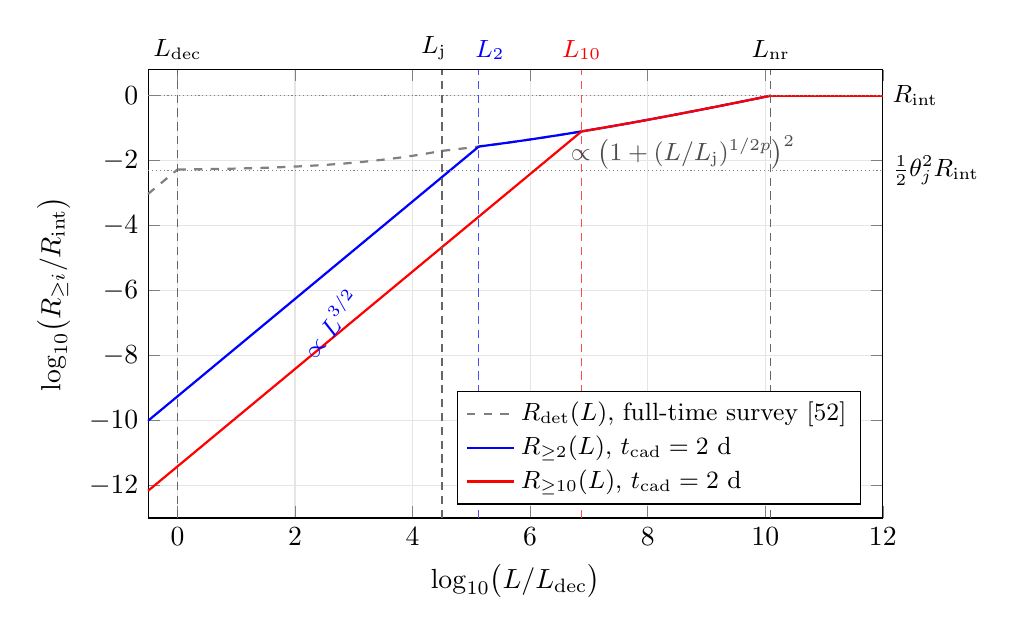
\begin{tikzpicture}
\begin{axis}[width=0.9\textwidth, height=0.6\textwidth, clip=false,
  xlabel={$\log_{10}\bigl(L/\Ldec\bigr)$}, ylabel={$\log_{10}\bigl(R_{\geq i}/\Rint\bigr)$},
  xmin=-0.5, xmax=12, ymin=-13, ymax=0.8,
  xtick={0,2,4,6,8,10,12}, ytick={-12,-10,-8,-6,-4,-2,0},
  grid=major, grid style={gray!20}, legend pos=south east, legend cell align=left,
  legend style={font=\small}, samples=200]
% full-time survey R_det(L) (thesis Eq. 52)
\addplot[gray, dashed, thick, domain=-0.5:0] {lgbase + 0.0270 + 1.5*x};
\addlegendentry{$\Rdet(L)$, full-time survey [52]}
\addplot[gray, dashed, thick, domain=0:4.5, forget plot] {logRtwo(x)};
\addplot[gray, dashed, thick, domain=4.5:10.0933, forget plot] {logRthree(x)};
\addplot[gray, dashed, thick, domain=10.0933:12, forget plot] {0};
% i = 2
\addplot[blue, thick, domain=-0.5:5.1275] {logRcad(x,xtwo,lqtwo)};
\addlegendentry{$R_{\geq2}(L)$, $\tcad=2$~d}
\addplot[blue, thick, domain=5.1275:10.0933, forget plot] {logRthree(x)};
\addplot[blue, thick, domain=10.0933:12, forget plot] {0};
% i = 10
\addplot[red, thick, domain=-0.5:6.8749] {logRcad(x,xten,lqten)};
\addlegendentry{$R_{\geq10}(L)$, $\tcad=2$~d}
\addplot[red, thick, domain=6.8749:10.0933, forget plot] {logRthree(x)};
\addplot[red, thick, domain=10.0933:12, forget plot] {0};
% horizontal reference levels
\draw[black!50, densely dotted] (axis cs:-0.5,0) -- (axis cs:12,0) node[right, black, font=\small] {$\Rint$};
\draw[black!50, densely dotted] (axis cs:-0.5,-2.30103) -- (axis cs:12,-2.30103) node[right, black, font=\small] {$\tfrac12\theta_j^2\Rint$};
% threshold luminosities
\draw[black!60, densely dashed] (axis cs:0,-13) -- (axis cs:0,0.8) node[above, black, font=\small] {$\Ldec$};
\draw[black!60, densely dashed] (axis cs:4.5,-13) -- (axis cs:4.5,0.8) node[above, black, font=\small, xshift=-3pt] {$\Lj$};
\draw[blue!70, densely dashed] (axis cs:5.1275,-13) -- (axis cs:5.1275,0.8) node[above, blue, font=\small, xshift=4pt] {$L_2$};
\draw[red!70, densely dashed] (axis cs:6.8749,-13) -- (axis cs:6.8749,0.8) node[above, red, font=\small] {$L_{10}$};
\draw[black!60, densely dashed] (axis cs:10.0933,-13) -- (axis cs:10.0933,0.8) node[above, black, font=\small] {$\Lnr$};
% slope labels
\node[blue, font=\small, rotate=52] at (axis cs:2.6,-7.0) {$\propto L^{3/2}$};
\node[black!70, font=\small] at (axis cs:8.6,-1.75) {$\propto\bigl(1+(L/\Lj)^{1/2p}\bigr)^2$};
\end{axis}
\end{tikzpicture}
\caption{The single-burst detection rate as a function of its luminosity, Eq.~\eqref{eq:RofL}, for the thesis parameters of Appendix~\ref{app:params} ($p=2.5$, $\Gamma_0\theta_j=10^{1.5}$, $\theta_j=0.1$, $\tj=10^4\,\tdec$) and a cadence of two days, for $i=2$ (blue) and $i=10$ (red). The dashed grey line is the full-time survey rate, thesis Eq.~52, which the $\geq i$ rates join at $L_i$. Below $L_i$ the rate is cadence-limited and rises as $L^{3/2}$; between $L_i$ and $\Lnr$ it is Euclidean-limited and grows only as the visible cone widens; above $\Lnr$ every burst inside $D_\Euc$ is detected. In these units the figure is independent of $\Flim$ and $D_\Euc$.}
\label{fig:RofL}
\end{figure}

\section{The full integral}
\label{sec:integral}

\subsection{Definition}

Each burst is now characterised by three quantities, $(q,D,L)$, distributed independently: $q$ and $D$ as before (uniform in volume and in $\cos\theta_{\rm obs}$), $L$ according to $\phi(L)$. The rate of events detected at least $i$ times is thesis Eq.~58 integrated over the luminosity distribution,
\begin{equation}
\label{eq:full3}
\Ravg=\int_{\Lmin}^{\Lmax}dL\,\phi(L)\;4\pi\theta_j^2\mathcal R\int_0^{q_\nr}dq\,q\int_0^{D_\Euc}dD\,D^2\;\Theta\Bigl(\frac{L\,\tF_p(q)}{4\pi D^2}-\Flim\Bigr)\,\Theta\bigl(t_+(D;L)-i\,\tcad\bigr),
\end{equation}
where, as in Section~\ref{sec:cadence}, the step approximation $P_{\geq i}\approx\Theta(\tau_{\rm det}-i)$ for $i\geq2$ has been used, and both the flux horizon and the cadence horizon now depend on $L$. Performing the $D$ integral with \eqref{eq:DmaxL} and \eqref{eq:DiL},
\begin{equation}
\label{eq:full2}
\Ravg=\theta_j^2\Rint\int_{\Lmin}^{\Lmax}dL\,\phi(L)\int_0^{q_\nr}dq\,q\;\min\Bigl(\tD_{\max}(q;L),\,\tD_i(L),\,1\Bigr)^3 ,
\end{equation}
the luminosity average of \eqref{eq:Rgeqi_exact}.

\subsection{The exact expression: integrating over luminosity first}
\label{sec:exact}

Both $L$-dependent distances in \eqref{eq:full2} scale as $L^{1/2}$, so their minimum does too,
\begin{equation}
\min\bigl(\tD_{\max}(q;L),\tD_i(L)\bigr)=\Bigl(\frac{L}{\Ldec}\Bigr)^{1/2}\min\bigl(\tF_p(q),\tF_p(q_i)\bigr)^{1/2}=\Bigl(\frac{L}{\Ldec}\Bigr)^{1/2}\tF_p\bigl(\max(q,q_i)\bigr)^{1/2},
\end{equation}
because $\tF_p$ decreases with $q$: at $q<q_i$ the cadence cap binds, at $q>q_i$ the flux horizon. With the threshold luminosity of the angle $\max(q,q_i)$ in the sense of \eqref{eq:LX}, $L_\Euc(q)\equiv\Ldec/\tF_p(q)$, the integrand is
\begin{equation}
\min\Bigl(\tD_{\max}(q;L),\tD_i(L),1\Bigr)^3=\begin{cases}\Bigl(\dfrac{L}{L_\Euc(\max(q,q_i))}\Bigr)^{3/2}, & L<L_\Euc(\max(q,q_i)),\\[8pt] 1, & L>L_\Euc(\max(q,q_i)),\end{cases}
\end{equation}
i.e. for a given angle, bursts fainter than $L_\Euc(\max(q,q_i))$ are seen out to a horizon inside the volume ($\propto L^{3/2}$ of them), brighter ones throughout the volume. The luminosity integral is therefore elementary for every $q$:
\begin{multline}
\label{eq:innerL}
\int_{\Lmin}^{\Lmax}dL\,\phi(L)\,\min\Bigl(\tD_{\max}(q;L),\tD_i(L),1\Bigr)^3
=\frac{\alpha+1}{\Lmax^{\alpha+1}-\Lmin^{\alpha+1}}\;\times\\
\Biggl[\;L_\Euc\bigl(\max(q,q_i)\bigr)^{-3/2}\;\frac{\min\bigl(\Lmax,L_\Euc(\max(q,q_i))\bigr)^{\alpha+5/2}-\Lmin^{\alpha+5/2}}{\alpha+5/2}\\
+\frac{\Lmax^{\alpha+1}-\max\bigl(\Lmin,L_\Euc(\max(q,q_i))\bigr)^{\alpha+1}}{\alpha+1}\Biggr],
\end{multline}
where each of the two terms is to be set to zero when its upper limit falls below its lower one (the first when $L_\Euc(\max(q,q_i))<\Lmin$, all bursts saturated; the second when $L_\Euc(\max(q,q_i))>\Lmax$, none saturated). Inserting \eqref{eq:innerL} into \eqref{eq:full2} leaves a single integral over $q$,
\begin{equation}
\label{eq:exactq}
\Ravg=\theta_j^2\Rint\int_0^{q_\nr}dq\,q\times\bigl[\text{Eq.~\eqref{eq:innerL}}\bigr],
\end{equation}
in which $L_\Euc(\max(q,q_i))$ is a piecewise power law in $\tq$ through \eqref{eq:Fp} ($\Ldec$ for $q<q_\dec$; $\Lj\,\tq^{2(p-1)}$ for $q_\dec<q<q_{\rm j}$; $\Lj\,\tq^{2p}$ for $q>q_{\rm j}$; constant $L_i$ for all $q<q_i$). Equation~\eqref{eq:exactq} is the exact analogue of thesis Eqs.~41--44: every piece is integrable in closed form, but the result is a long sum of incomplete powers of the various $\tq$ boundaries (with $\Lmin$ and $\Lmax$ now cutting the $q$ range at the angles where $L_\Euc(q)=\Lmin$ and $L_\Euc(q)=\Lmax$). It is the appropriate starting point for a numerical evaluation. As in the thesis, we proceed with the most-contributing-point approximation instead, which gives compact analytic results; in the cases we checked it reproduces \eqref{eq:exactq} to within $5$--$25\%$, comparable to its accuracy for a single luminosity (thesis Fig.~11).

\subsection{Reduction to one dimension}

The most-contributing-point approximation replaces the $q$ integral in \eqref{eq:full2}, for each luminosity separately, by $R_{\geq i}(L)$ of Eq.~\eqref{eq:RofL}. Since the regime of a burst is set by its luminosity alone (Eq.~\eqref{eq:switch}), the average is a one-dimensional integral over a piecewise power law:
\begin{equation}
\label{eq:oneD}
\boxed{\;\Ravg=\int_{\Lmin}^{\Lmax}\phi(L)\,R_{\geq i}(L)\,dL\;}
\end{equation}
with $\phi$ from \eqref{eq:phi} and $R_{\geq i}(L)$ from \eqref{eq:RofL}. The rest of the derivation is the evaluation of this integral.

\section{Analytic solution, case by case}
\label{sec:solution}

\subsection{The elementary integral}

Every term in \eqref{eq:oneD} is of the form $\int L^{\alpha}\cdot L^{\beta}\,dL$ with $\beta\in\{\tfrac32,\ \tfrac{1}{2(p-1)},\ \tfrac1{p-1},\ \tfrac1{2p},\ \tfrac1p,\ 0\}$, for which
\begin{equation}
\label{eq:elem}
\int_a^b L^{\alpha+\beta}\,dL=\begin{cases}\dfrac{b^{\alpha+\beta+1}-a^{\alpha+\beta+1}}{\alpha+\beta+1}, & \alpha+\beta\neq-1,\\[8pt] \ln\dfrac{b}{a}, & \alpha+\beta=-1 .\end{cases}
\end{equation}
The logarithmic case occurs at isolated values of $\alpha$ (e.g. $\alpha=-5/2$ for the cadence-limited term, $\alpha=-1$ for the saturated term and for the normalisation of $\phi$); they are collected in Appendix~\ref{app:logs} and are the continuous limits of the general expressions.

\subsection{The four segments}
\label{sec:segments}

The integration range $[\Lmin,\Lmax]$ is cut by the thresholds $L_i$, $\Lj$, $\Lnr$ into at most four segments, on each of which $R_{\geq i}(L)$ is one line of Eq.~\eqref{eq:RofL}. Writing $[a,b]$ for the overlap of a segment with $[\Lmin,\Lmax]$ (a segment whose overlap is empty contributes nothing), the contributions are:

\medskip\noindent\textbf{Cadence-limited segment,} with $a=\Lmin$ and $b=\min(\Lmax,L_i)$. Here $\phi R\propto L^{\alpha+3/2}$:
\begin{equation}
\label{eq:seg1}
\int_a^b\phi(L)\,R_{\geq i}(L)\,dL=\tfrac12\theta_j^2\min(q_i,q_\nr)^2\Rint\;\frac{\alpha+1}{\Lmax^{\alpha+1}-\Lmin^{\alpha+1}}\;L_i^{-3/2}\;\frac{b^{\alpha+5/2}-a^{\alpha+5/2}}{\alpha+5/2}.
\end{equation}
It is the single-luminosity result $\tfrac12\theta_j^2\min(q_i,q_\nr)^2\tD_i^3\Rint$ with $\tD_i^3=(L/L_i)^{3/2}$ replaced by its average over the segment.

\medskip\noindent\textbf{Euclidean-limited segment, phase II} (exists only if $q_i<q_{\rm j}$), with $a=\max(\Lmin,L_i)$ and $b=\min(\Lmax,\Lj)$. Expanding the square in the second line of \eqref{eq:RofL},
\begin{equation}
\Bigl(1+\Bigl(\frac{L}{\Lj}\Bigr)^{\frac{1}{2(p-1)}}\Bigr)^2=1+2\Bigl(\frac{L}{\Lj}\Bigr)^{\frac{1}{2(p-1)}}+\Bigl(\frac{L}{\Lj}\Bigr)^{\frac{1}{p-1}},
\end{equation}
gives three elementary integrals:
\begin{multline}
\label{eq:seg2}
\int_a^b\phi(L)\,R_{\geq i}(L)\,dL=\tfrac12\theta_j^2\Rint\;\frac{\alpha+1}{\Lmax^{\alpha+1}-\Lmin^{\alpha+1}}\Biggl[\frac{b^{\alpha+1}-a^{\alpha+1}}{\alpha+1}\\
+2\,\Lj^{-\frac{1}{2(p-1)}}\;\frac{b^{\alpha+1+\frac{1}{2(p-1)}}-a^{\alpha+1+\frac{1}{2(p-1)}}}{\alpha+1+\frac{1}{2(p-1)}}
+\Lj^{-\frac{1}{p-1}}\;\frac{b^{\alpha+1+\frac{1}{p-1}}-a^{\alpha+1+\frac{1}{p-1}}}{\alpha+1+\frac{1}{p-1}}\Biggr].
\end{multline}

\medskip\noindent\textbf{Euclidean-limited segment, phase III} (exists only if $q_i<q_\nr$), with $a=\max(\Lmin,L_i,\Lj)$ and $b=\min(\Lmax,\Lnr)$. In the same way,
\begin{multline}
\label{eq:seg3}
\int_a^b\phi(L)\,R_{\geq i}(L)\,dL=\tfrac12\theta_j^2\Rint\;\frac{\alpha+1}{\Lmax^{\alpha+1}-\Lmin^{\alpha+1}}\Biggl[\frac{b^{\alpha+1}-a^{\alpha+1}}{\alpha+1}\\
+2\,\Lj^{-\frac{1}{2p}}\;\frac{b^{\alpha+1+\frac{1}{2p}}-a^{\alpha+1+\frac{1}{2p}}}{\alpha+1+\frac{1}{2p}}
+\Lj^{-\frac{1}{p}}\;\frac{b^{\alpha+1+\frac{1}{p}}-a^{\alpha+1+\frac{1}{p}}}{\alpha+1+\frac{1}{p}}\Biggr].
\end{multline}

\medskip\noindent\textbf{Saturated segment,} with $a=\max(\Lmin,L_i,\Lnr)$ and $b=\Lmax$. Here $R_{\geq i}=\Rint$ and the contribution is $\Rint$ times the fraction of the population in the segment:
\begin{equation}
\label{eq:seg4}
\int_a^b\phi(L)\,R_{\geq i}(L)\,dL=\Rint\;\frac{b^{\alpha+1}-a^{\alpha+1}}{\Lmax^{\alpha+1}-\Lmin^{\alpha+1}} .
\end{equation}

\medskip\noindent The full result is the sum of \eqref{eq:seg1}--\eqref{eq:seg4}. (The prefactor $\tfrac12\theta_j^2q_\nr^2=1$ makes \eqref{eq:seg4} consistent with the other three.) We now write it out for the configurations that occur in practice.

\subsection{Assembled results}
\label{sec:cases}

\noindent\textbf{Case A: all bursts cadence-limited,} $\Lmax\le L_i$. This is the situation of a survey whose flux limit is high compared with the population (range~I--II of the thesis for every burst). Only \eqref{eq:seg1} contributes, with $a=\Lmin$, $b=\Lmax$:
\begin{multline}
\label{eq:caseA}
\Ravg=\tfrac12\theta_j^2\min(q_i,q_\nr)^2\Rint\;L_i^{-3/2}\;\frac{\alpha+1}{\alpha+5/2}\;\frac{\Lmax^{\alpha+5/2}-\Lmin^{\alpha+5/2}}{\Lmax^{\alpha+1}-\Lmin^{\alpha+1}}\\
=R_{\geq i}\bigl(L_{\rm eff}\bigr),\qquad\text{with}\qquad L_{\rm eff}^{3/2}\equiv\int_{\Lmin}^{\Lmax}\phi(L)\,L^{3/2}\,dL .
\end{multline}
The single-luminosity formula survives with $L$ replaced by the effective luminosity $L_{\rm eff}=\langle L^{3/2}\rangle^{2/3}$, the volume-weighted mean. For a broad distribution, $\Lmax\gg\Lmin$, its three limits are
\begin{equation}
\label{eq:caseAlimits}
\Ravg\approx\begin{cases}
\dfrac{\alpha+1}{\alpha+5/2}\,R_{\geq i}(\Lmax), & \alpha>-1,\\[10pt]
\dfrac{|\alpha+1|}{\alpha+5/2}\,R_{\geq i}(\Lmax)\Bigl(\dfrac{\Lmin}{\Lmax}\Bigr)^{|\alpha+1|}=\dfrac{|\alpha+1|}{\alpha+5/2}\,R_{\geq i}(\Lmin)\Bigl(\dfrac{\Lmax}{\Lmin}\Bigr)^{\alpha+5/2}, & -\tfrac52<\alpha<-1,\\[10pt]
\dfrac{|\alpha+1|}{|\alpha+5/2|}\,R_{\geq i}(\Lmin), & \alpha<-\tfrac52 .
\end{cases}
\end{equation}
The bright end dominates for $\alpha>-1$ and the faint end for $\alpha<-5/2$. In the middle range both ends matter: the rate is $R_{\geq i}(\Lmax)$ suppressed by the small fraction of bursts that are bright, $\sim(\Lmin/\Lmax)^{|\alpha+1|}$, or equivalently $R_{\geq i}(\Lmin)$ boosted by the volume factor of the bright tail, $(\Lmax/\Lmin)^{\alpha+5/2}$.

\medskip\noindent\textbf{Case B: the distribution straddles $L_i$, no saturation,} $\Lmin<L_i<\Lmax\le\Lnr$. This is the generic situation for $i\geq2$ with a daily cadence: the fiducial burst sits near $L_i$, and the population extends to both sides. For $q_{\rm j}<q_i<q_\nr$ (the cadence angle beyond the jet-break angle, as for $i\geq2$ and $\tcad\gtrsim1$~d in Fig.~\ref{fig:RofL}) the phase-II segment is absent and \eqref{eq:seg1}~+~\eqref{eq:seg3} give
\begin{multline}
\label{eq:caseB}
\Ravg=\tfrac12\theta_j^2\Rint\;\frac{\alpha+1}{\Lmax^{\alpha+1}-\Lmin^{\alpha+1}}\Biggl[\;q_i^2\,L_i^{-3/2}\;\frac{L_i^{\alpha+5/2}-\Lmin^{\alpha+5/2}}{\alpha+5/2}
\;+\;\frac{\Lmax^{\alpha+1}-L_i^{\alpha+1}}{\alpha+1}\\
+2\,\Lj^{-\frac{1}{2p}}\;\frac{\Lmax^{\alpha+1+\frac{1}{2p}}-L_i^{\alpha+1+\frac{1}{2p}}}{\alpha+1+\frac{1}{2p}}
\;+\;\Lj^{-\frac{1}{p}}\;\frac{\Lmax^{\alpha+1+\frac{1}{p}}-L_i^{\alpha+1+\frac{1}{p}}}{\alpha+1+\frac{1}{p}}\Biggr],
\end{multline}
where $q_i^2=\bigl(1+(L_i/\Lj)^{1/(2p)}\bigr)^2$ by \eqref{eq:qEucL}, so that the cadence-limited and Euclidean-limited parts join continuously at $L_i$. The first term collects the bursts fainter than $L_i$, whose horizon lies inside the volume; the remaining three collect the brighter bursts, which are seen throughout the volume within the widening cone $q_\Euc(L)$. If instead $q_\dec<q_i<q_{\rm j}$ (short cadence or small $i$, so that $L_i<\Lj$), the phase-II segment \eqref{eq:seg2} over $[L_i,\min(\Lmax,\Lj)]$ is inserted between the two, and the phase-III segment starts at $\Lj$.

\medskip\noindent\textbf{Case C: the bright end saturates,} $\Lmax>\Lnr$. The phase-III segment is cut at $\Lnr$ and the saturated segment \eqref{eq:seg4} is added; for $\Lmin<L_i$ and $q_{\rm j}<q_i<q_\nr$,
\begin{multline}
\label{eq:caseC}
\Ravg=\tfrac12\theta_j^2\Rint\;\frac{\alpha+1}{\Lmax^{\alpha+1}-\Lmin^{\alpha+1}}\Biggl[\;q_i^2\,L_i^{-3/2}\;\frac{L_i^{\alpha+5/2}-\Lmin^{\alpha+5/2}}{\alpha+5/2}
\;+\;\frac{\Lnr^{\alpha+1}-L_i^{\alpha+1}}{\alpha+1}\\
+2\,\Lj^{-\frac{1}{2p}}\;\frac{\Lnr^{\alpha+1+\frac{1}{2p}}-L_i^{\alpha+1+\frac{1}{2p}}}{\alpha+1+\frac{1}{2p}}
\;+\;\Lj^{-\frac{1}{p}}\;\frac{\Lnr^{\alpha+1+\frac{1}{p}}-L_i^{\alpha+1+\frac{1}{p}}}{\alpha+1+\frac{1}{p}}\Biggr]\\
\;+\;\Rint\;\frac{\Lmax^{\alpha+1}-\Lnr^{\alpha+1}}{\Lmax^{\alpha+1}-\Lmin^{\alpha+1}} .
\end{multline}
The last term is the fraction of the population brighter than $\Lnr$, each of which is detected with certainty. For $\alpha>-1$ and $\Lmax\gg\Lnr$ this fraction tends to one and $\Ravg\to\Rint$; for $\alpha<-1$ it is a small number $\approx(\Lmin/\Lnr)^{|\alpha+1|}$.

\medskip\noindent\textbf{Case D: the single-luminosity limit,} $\Lmax\to\Lmin$. Then $\phi\to\delta(L-\Lmin)$ and \eqref{eq:oneD} gives $R_{\geq i}(\Lmin)$. Explicitly, in \eqref{eq:caseA}, $\frac{\alpha+1}{\alpha+5/2}\,\frac{\Lmax^{\alpha+5/2}-\Lmin^{\alpha+5/2}}{\Lmax^{\alpha+1}-\Lmin^{\alpha+1}}\to\Lmin^{3/2}$ by l'H\^opital's rule, and likewise for every other segment: the results of the thesis are recovered exactly.

\subsection{Power-law description and which luminosities dominate}
\label{sec:dominance}

Following thesis Eqs.~53 and 77, we drop the ``$+1$'' in the Euclidean-limited lines of \eqref{eq:RofL} where $\tq_\Euc\gg1$ (phase III) and keep only the ``$1$'' where $\tq_\Euc\ll1$ (phase II), so that each line is a pure power of $L$:
\begin{equation}
\label{eq:RofLpow}
R_{\geq i}(L)\approx\tfrac12\theta_j^2\Rint\times\begin{cases}
q_i^2\,(L/L_i)^{3/2}, & L<L_i,\\[3pt]
1, & L_i<L<\Lj\ (\text{if }q_i<q_{\rm j}),\\[3pt]
(L/\Lj)^{1/p}, & \max(L_i,\Lj)<L<\Lnr,\\[3pt]
2\theta_j^{-2}, & L>\Lnr .
\end{cases}
\end{equation}
The integrand of \eqref{eq:oneD} is then $\phi(L)R_{\geq i}(L)\propto L^{\alpha+3/2}$ below $L_i$, $\propto L^{\alpha}$ or $L^{\alpha+1/p}$ in the Euclidean-limited range, and $\propto L^{\alpha}$ once saturated. Reading off where each power rises or falls gives three regimes (Fig.~\ref{fig:dens}):

\begin{center}\small
\renewcommand{\arraystretch}{1.35}
\begin{tabular}{l l p{7.6cm}}
\toprule
index & integrand $\phi(L)R_{\geq i}(L)$ & detections dominated by \\
\midrule
$\alpha<-\tfrac52$ & falls everywhere & the faint end $\Lmin$: many faint bursts seen in a small volume \\
$-\tfrac52<\alpha<-1$ & rises below $L_i$, falls above & the knee $L_i$: bursts whose cadence horizon just reaches $D_\Euc$ \\
$\alpha>-1$ & rises everywhere (until saturation) & the bright end $\Lmax$: few bright bursts seen throughout the volume \\
\bottomrule
\end{tabular}
\end{center}

\noindent (For $-1-1/p<\alpha<-1$ the phase-III integrand $\propto L^{\alpha+1/p}$ rises slowly, so the bright end competes with the knee unless $\Lmax$ is close to $L_i$; the boundary between the last two regimes is therefore soft.) The three regimes have different leading-order results, which are the analytic content of the luminosity distribution:

\medskip\noindent\emph{Faint-end dominated,} $\alpha<-5/2$: from \eqref{eq:caseAlimits},
\begin{equation}
\label{eq:faint}
\Ravg\approx\frac{|\alpha+1|}{|\alpha+5/2|}\,R_{\geq i}(\Lmin)\qquad(\Lmin\ll L_i),
\end{equation}
the single-luminosity rate at $\Lmin$ with an order-unity factor; all scalings with $\Flim$ and $\tcad$ are those of thesis Eq.~77.

\medskip\noindent\emph{Knee dominated,} $-5/2<\alpha<-1$ and $\Lmin\ll L_i\ll\Lmax$: keeping the leading term of each bracket in \eqref{eq:caseB} (the $L_i^{\alpha+5/2}$ term of the first and the $L_i^{\alpha+1}$ terms of the others, both of which are the values at the knee),
\begin{equation}
\label{eq:knee}
\Ravg\approx\tfrac12\theta_j^2q_i^2\Rint\;\frac{(\alpha+1)\,L_i^{\alpha+1}}{\Lmax^{\alpha+1}-\Lmin^{\alpha+1}}\Bigl[\frac{1}{\alpha+5/2}+\frac{1}{|\alpha+1|}\Bigr]
\approx R_{\geq i}(L_i)\Bigl(1+\frac{|\alpha+1|}{\alpha+5/2}\Bigr)\Bigl(\frac{\Lmin}{L_i}\Bigr)^{|\alpha+1|},
\end{equation}
where the second form uses $\Lmax^{\alpha+1}\ll\Lmin^{\alpha+1}$. For $\alpha=-2$ this is $\Ravg\approx3\,R_{\geq i}(L_i)\,\Lmin/L_i$: the rate is that of a burst at the knee, $R_{\geq i}(L_i)=\tfrac12\theta_j^2q_i^2\Rint$ (which is independent of $\Flim$), times the fraction of the population within a factor of a few of the knee. In the cases of Fig.~\ref{fig:dens} the approximation \eqref{eq:knee} is within $10\%$ of the full expression \eqref{eq:caseB}.

The consequences for the survey scalings are the most important result of this section. Since $R_{\geq i}(L_i)$ does not depend on $\Flim$ and $L_i\propto\Flim$ (Eq.~\eqref{eq:Li}),
\begin{equation}
\label{eq:kneescaling}
\Ravg\;\propto\;q_i^2\,L_i^{\alpha+1}\;\propto\;\Flim^{\,\alpha+1}\;\Bigl(\frac{i\,\tcad}{\tj}\Bigr)^{1+p(\alpha+1)}\qquad(i\,\tcad>\tj,\ \text{knee dominated}),
\end{equation}
to be compared with the single-luminosity $R_{\geq i}\propto\Flim^{-3/2}(i\,\tcad/\tj)^{-3(p-2)/2}$ of thesis Eq.~77. For $\alpha=-2$ and $p=2.5$ the dependence on the limiting flux softens from $\Flim^{-3/2}$ to $\Flim^{-1}$ -- lowering the flux limit by a factor ten gains a factor ten in detections instead of thirty -- while the dependence on the cadence steepens from $(i\,\tcad)^{-0.75}$ to $(i\,\tcad)^{-1.5}$. The reason is that a deeper limit no longer enlarges the volume in which a fixed burst is seen; it lowers the knee $L_i$, admitting the more numerous fainter bursts at the rate $\phi(L_i)L_i\propto L_i^{\alpha+1}$.

\medskip\noindent\emph{Bright-end dominated,} $\alpha>-1$: for $\Lmax<\Lnr$ the last bracket of \eqref{eq:caseB} dominates and
\begin{equation}
\label{eq:bright}
\Ravg\approx\frac{\alpha+1}{\alpha+1+1/p}\,R_{\geq i}(\Lmax)\qquad(L_i\ll\Lmax<\Lnr),
\end{equation}
while for $\Lmax\gg\Lnr$ the saturated term of \eqref{eq:caseC} takes over and $\Ravg\to\Rint$: essentially every burst inside $D_\Euc$ is bright enough to be seen from anywhere inside the volume.

\begin{figure}[t]
\centering
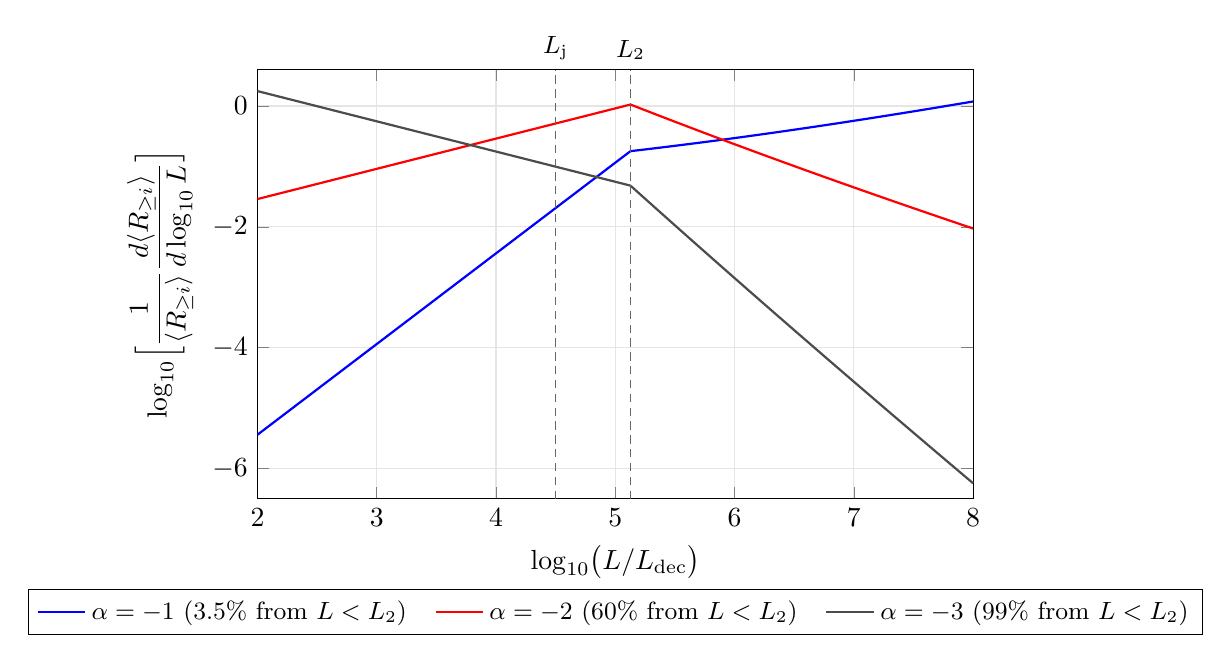
\begin{tikzpicture}
\begin{axis}[width=0.88\textwidth, height=0.58\textwidth, clip=false,
  xlabel={$\log_{10}\bigl(L/\Ldec\bigr)$}, ylabel={$\log_{10}\Bigl[\dfrac{1}{\Ravg}\dfrac{d\Ravg}{d\log_{10}L}\Bigr]$},
  xmin=2, xmax=8, ymin=-6.5, ymax=0.6,
  grid=major, grid style={gray!20}, legend cell align=left, legend columns=3,
  legend style={font=\small, at={(0.5,-0.21)}, anchor=north, /tikz/every even column/.append style={column sep=0.8em}},
  samples=200]
% alpha = -1 : log10(L phi) = -1.1403 ; log10 <R>/R_int = -1.5950
\addplot[blue, thick, domain=2:5.1275] {0.36222 - 1.1403 + logRcad(x,xtwo,lqtwo) + 1.5950};
\addlegendentry{$\alpha=-1$ (3.5\% from $L<L_2$)}
\addplot[blue, thick, domain=5.1275:8, forget plot] {0.36222 - 1.1403 + logRthree(x) + 1.5950};
% alpha = -2 : log10(L phi) = 2 - x ; log10 <R>/R_int = -4.3533
\addplot[red, thick, domain=2:5.1275] {0.36222 + 2 - x + logRcad(x,xtwo,lqtwo) + 4.3533};
\addlegendentry{$\alpha=-2$ (60\% from $L<L_2$)}
\addplot[red, thick, domain=5.1275:8, forget plot] {0.36222 + 2 - x + logRthree(x) + 4.3533};
% alpha = -3 : log10(L phi) = 4.30103 - 2x ; log10 <R>/R_int = -5.8383
\addplot[black!70, thick, domain=2:5.1275] {0.36222 + 4.30103 - 2*x + logRcad(x,xtwo,lqtwo) + 5.8383};
\addlegendentry{$\alpha=-3$ (99\% from $L<L_2$)}
\addplot[black!70, thick, domain=5.1275:8, forget plot] {0.36222 + 4.30103 - 2*x + logRthree(x) + 5.8383};
% thresholds
\draw[black!60, densely dashed] (axis cs:4.5,-6.5) -- (axis cs:4.5,0.6) node[above, black, font=\small] {$\Lj$};
\draw[black!60, densely dashed] (axis cs:5.1275,-6.5) -- (axis cs:5.1275,0.6) node[above, black, font=\small] {$L_2$};
\end{axis}
\end{tikzpicture}
\caption{Where the detections come from: the detected-luminosity density per decade, normalised to the total rate, for $i=2$, $\tcad=2$~d, the thesis parameters, and a population spanning $\Lmin=10^{2}\Ldec$ to $\Lmax=10^{8}\Ldec$ with three values of $\alpha$. The slope is $\alpha+5/2$ below the knee $L_2$ and $\alpha+1+1/p$ above it. For $\alpha=-3$ the faint end dominates, for $\alpha=-2$ the bursts near the knee, for $\alpha=-1$ the bright end. The percentages are the fractions of $\Ravg$ contributed by bursts fainter than $L_2$ (from Eqs.~\eqref{eq:seg1} and \eqref{eq:seg3}); the normalisations are listed in Appendix~\ref{app:params}.}
\label{fig:dens}
\end{figure}

\section{The luminosities of the detected bursts}
\label{sec:detected}

The integrand of \eqref{eq:oneD} is itself an observable: the distribution of luminosities among the \emph{detected} bursts,
\begin{equation}
\label{eq:dRdL}
\frac{d\Ravg}{dL}=\phi(L)\,R_{\geq i}(L),\qquad\text{or per decade}\qquad \frac{d\Ravg}{d\log_{10}L}=\ln(10)\,L\,\phi(L)\,R_{\geq i}(L),
\end{equation}
which is the intrinsic distribution re-weighted by the detection volume. Below the knee the weight is $L^{3/2}$: with $\alpha=-2$ the intrinsic population per decade falls as $L^{-1}$ while the detected one \emph{rises} as $L^{1/2}$ up to $L_i$ (Fig.~\ref{fig:dens}). The detected sample is therefore strongly biased towards luminous bursts (the Malmquist bias of a flux-limited survey), and the median luminosity of the detected bursts,
\begin{equation}
\int_{\Lmin}^{L_{\rm med,det}}\phi(L)\,R_{\geq i}(L)\,dL=\tfrac12\Ravg ,
\end{equation}
lies far above the population median \eqref{eq:Lmedpop}. In case~A (all cadence-limited) it is explicit,
\begin{equation}
\label{eq:LmedA}
L_{\rm med,det}^{\ \alpha+5/2}=\tfrac12\bigl(\Lmin^{\alpha+5/2}+\Lmax^{\alpha+5/2}\bigr)\qquad(\Lmax\le L_i),
\end{equation}
which for $\alpha=-2$ and $\Lmax\gg\Lmin$ gives $L_{\rm med,det}\approx\Lmax/4$, against $L_{\rm med,pop}=2\Lmin$. In the general case the median is found segment by segment from \eqref{eq:seg1}--\eqref{eq:seg4}; for the $\alpha=-2$ example of Fig.~\ref{fig:dens} it is $L_{\rm med,det}\approx10^{5.0}\Ldec$, three orders of magnitude above $L_{\rm med,pop}=10^{2.3}\Ldec$, and just below the knee $L_2=10^{5.1}\Ldec$.

Conversely, the \emph{effective luminosity} at which the single-luminosity model of the thesis reproduces the population rate, $R_{\geq i}(L_{\rm eff})=\Ravg$, is obtained by inverting \eqref{eq:RofL}. In case~A it is the volume-weighted mean $L_{\rm eff}=\langle L^{3/2}\rangle^{2/3}$ of \eqref{eq:caseA}; in the knee-dominated regime, where $\Ravg<R_{\geq i}(L_i)$, it lies on the rising branch and \eqref{eq:knee} gives
\begin{equation}
\label{eq:Leff}
L_{\rm eff}\approx L_i\Bigl[\Bigl(1+\frac{|\alpha+1|}{\alpha+5/2}\Bigr)\Bigl(\frac{\Lmin}{L_i}\Bigr)^{|\alpha+1|}\Bigr]^{2/3}\qquad(-\tfrac52<\alpha<-1),
\end{equation}
e.g. $L_{\rm eff}\approx L_i\,(3\Lmin/L_i)^{2/3}$ for $\alpha=-2$ (for the example of Fig.~\ref{fig:dens}, $L_{\rm eff}\approx10^{3.4}\Ldec$). Note that $L_{\rm eff}$ depends on the survey through $L_i\propto\Flim\,(i\,\tcad)^{p}$: no single luminosity reproduces the population rate for all surveys, which is the quantitative statement of why a distribution is needed.

\section{Summary of results}
\label{sec:summary}

\noindent\textbf{Model.} Identical light-curve shapes; luminosities $L\equiv\Lnu$ distributed as $\phi(L)\propto L^{\alpha}$ on $[\Lmin,\Lmax]$, normalised so that $\Rint$ is the total GRB rate inside $D_\Euc$. Survey with limiting flux $\Flim$ and cadence $\tcad$; at least $i\geq2$ detections required; $q_\dec<q_i$; step approximation for $P_{\geq i}$; most-contributing-point approximation for the $(q,D)$ integral.

\noindent\textbf{Scalings.} Luminosity enters only through $\tFlim=\Ldec/L$ with $\Ldec=4\pi D_\Euc^2\Flim$. All distances scale as $L^{1/2}$; all angles and times except $q_\Euc(L)$ are fixed. The regime of a burst is set by its luminosity relative to the threshold luminosities $L_X=\Ldec/\tF_p(q_X)$ at which $q_\Euc(L_X)=q_X$:
\begin{gather*}
\Ldec=4\pi D_\Euc^2\Flim,\qquad \Lj=\Ldec(\Gamma_0\theta_j)^{2(p-1)},\qquad \Lnr=\Lj\,\tq_\nr^{\,2p},\\
L_i=\frac{\Ldec}{\tF_\nu(i\,\tcad)}=\Lj\Bigl(\frac{i\,\tcad}{\tj}\Bigr)^{p}\quad(i\,\tcad>\tj).
\end{gather*}

\noindent\textbf{Single-burst rate} (Eq.~\eqref{eq:RofL}):
\[
R_{\geq i}(L)=\tfrac12\theta_j^2\Rint\times\begin{cases}\min(q_i,q_\nr)^2\,(L/L_i)^{3/2}, & L<L_i,\\[2pt] \bigl(1+(L/\Lj)^{1/(2(p-1))}\bigr)^2, & L_i<L<\Lj,\\[2pt] \bigl(1+(L/\Lj)^{1/(2p)}\bigr)^2, & \max(L_i,\Lj)<L<\Lnr,\\[2pt] 2\theta_j^{-2}, & L>\max(L_i,\Lnr).\end{cases}
\]

\noindent\textbf{Population rate} (Eq.~\eqref{eq:oneD}): $\Ravg=\int\phi(L)R_{\geq i}(L)\,dL$, evaluated in closed form as the sum of the segment contributions \eqref{eq:seg1}--\eqref{eq:seg4}; assembled results for the practical cases in Eqs.~\eqref{eq:caseA}, \eqref{eq:caseB}, \eqref{eq:caseC}. The exact (non-approximated) rate is the single $q$ integral \eqref{eq:exactq} with the closed-form luminosity integral \eqref{eq:innerL}.

\noindent\textbf{Which bursts are detected.} $\alpha<-5/2$: the faint end, $\Ravg\approx\frac{|\alpha+1|}{|\alpha+5/2|}R_{\geq i}(\Lmin)$. $-5/2<\alpha<-1$: the knee, $\Ravg\approx R_{\geq i}(L_i)\bigl(1+\frac{|\alpha+1|}{\alpha+5/2}\bigr)(\Lmin/L_i)^{|\alpha+1|}\propto\Flim^{\alpha+1}(i\,\tcad/\tj)^{1+p(\alpha+1)}$. $\alpha>-1$: the bright end, $\Ravg\approx\frac{\alpha+1}{\alpha+1+1/p}R_{\geq i}(\Lmax)$, saturating at $\Rint$ once $\Lmax\gg\Lnr$. The detected luminosities follow $\phi(L)R_{\geq i}(L)$ and are strongly biased towards the knee and above.

\noindent\textbf{Limitations.} The gray assumption ignores the co-variation of $\tdec$ and $\tj$ with the energy; the step approximation for $P_{\geq i}$ and the most-contributing-point approximation carry the same few-tens-of-per-cent accuracy as in the thesis; the case $q_i<q_\dec$ ($i\,\tcad<\tdec$) is excluded; and, as in the thesis, the universe is Euclidean with a sharp edge at $D_\Euc$.

\appendix

\section{The logarithmic special cases}
\label{app:logs}

Whenever an exponent in \eqref{eq:elem} equals $-1$ the power bracket is replaced by a logarithm; each such case is the continuous limit of the general formula and no result changes discontinuously. The values of $\alpha$ concerned and the replacements are:

\begin{center}\small
\renewcommand{\arraystretch}{1.4}
\begin{tabular}{l p{5.4cm} l}
\toprule
value of $\alpha$ & where it appears & replacement \\
\midrule
$\alpha=-1$ & normalisation of $\phi$; ``$1$'' terms of \eqref{eq:seg2}, \eqref{eq:seg3}; saturated segment \eqref{eq:seg4} & $\dfrac{b^{\alpha+1}-a^{\alpha+1}}{\alpha+1}\to\ln\dfrac{b}{a}$ \\
$\alpha=-\tfrac52$ & cadence-limited segment \eqref{eq:seg1} & $\dfrac{b^{\alpha+5/2}-a^{\alpha+5/2}}{\alpha+5/2}\to\ln\dfrac{b}{a}$ \\
$\alpha=-1-\tfrac{1}{2(p-1)}$,\ $-1-\tfrac{1}{p-1}$ & cross and square terms of the phase-II segment \eqref{eq:seg2} & the corresponding bracket $\to\ln\dfrac{b}{a}$ \\
$\alpha=-1-\tfrac{1}{2p}$,\ $-1-\tfrac{1}{p}$ & cross and square terms of the phase-III segment \eqref{eq:seg3} & the corresponding bracket $\to\ln\dfrac{b}{a}$ \\
\bottomrule
\end{tabular}
\end{center}

\noindent For example, at $\alpha=-1$ the distribution is $\phi(L)=1/(L\ln(\Lmax/\Lmin))$ and case~A becomes
\[
\Ravg=\tfrac12\theta_j^2\min(q_i,q_\nr)^2\Rint\,L_i^{-3/2}\;\frac{2}{3}\;\frac{\Lmax^{3/2}-\Lmin^{3/2}}{\ln(\Lmax/\Lmin)}\qquad(\alpha=-1),
\]
while at $\alpha=-5/2$ it becomes
\[
\Ravg=\tfrac12\theta_j^2\min(q_i,q_\nr)^2\Rint\,L_i^{-3/2}\;\frac{3}{2}\;\frac{\ln(\Lmax/\Lmin)}{\Lmin^{-3/2}-\Lmax^{-3/2}}\qquad(\alpha=-\tfrac52).
\]

\section{Parameters used in the figures}
\label{app:params}

Both figures use the thesis parameters (thesis footnote~4): $p=2.5$, $\Gamma_0=10^{2.5}$, $\theta_j=0.1$~rad, $E_{\rm k,iso}=10^{53}$~erg, $n=1$~cm$^{-3}$, giving $\tdec=19.4$~s, $\ttj=10^4$ ($\tj=2.24$~d), $\tq_\dec=(\Gamma_0\theta_j)^{-1}=10^{-1.5}$, $q_\dec=1.032$, $q_\nr=14.14$, $\tq_\nr=13.14$, and $\tfrac12\theta_j^2=10^{-2.30}$. The threshold luminosities in units of $\Ldec$ are then, from \eqref{eq:Lj}--\eqref{eq:Li},
\[
\frac{\Lj}{\Ldec}=(\Gamma_0\theta_j)^{2(p-1)}=10^{4.50},\qquad
\frac{\Lnr}{\Ldec}=\frac{\Lj}{\Ldec}\,\tq_\nr^{\,2p}=10^{10.09},
\]
(reproducing $\tF_{\rm lim,j}=10^{-4.5}$ and $\tF_{\rm lim,nr}=10^{-10.1}$ of thesis Fig.~11), and for $\tcad=2$~d
\begin{gather*}
i=2:\quad \frac{i\,\tcad}{\tj}=1.78,\quad q_2=2.335,\quad \frac{L_2}{\Ldec}=10^{5.13};\\
i=10:\quad \frac{i\,\tcad}{\tj}=8.91,\quad q_{10}=3.985,\quad \frac{L_{10}}{\Ldec}=10^{6.87}.
\end{gather*}
(With $\tcad=1$~d and $i=2$ one has $i\,\tcad<\tj$, $q_2=1.958$ just inside phase~II, and $L_2=10^{4.44}\Ldec$ practically coincides with $\Lj$; the two-day cadence was chosen to separate the two thresholds in the figure.) In Fig.~\ref{fig:dens} the population spans $[\Lmin,\Lmax]=[10^{2},10^{8}]\,\Ldec$; the total rates from Eq.~\eqref{eq:caseB} are $\Ravg/\Rint=2.54\times10^{-2}$, $4.43\times10^{-5}$ and $1.45\times10^{-6}$ for $\alpha=-1,-2,-3$, to be compared with $R_{\geq2}(L_2)/\Rint=1.82\times10^{-2}$ for a single burst at the knee; the fractions contributed by $L<L_2$ are $3.5\%$, $59.5\%$ and $99.2\%$; the detected medians are $10^{6.9}$, $10^{5.0}$, $10^{2.5}\Ldec$ against population medians of $10^{5.0}$, $10^{2.3}$, $10^{2.15}\Ldec$; and the knee approximation \eqref{eq:knee} for $\alpha=-2$ is $0.92$ of the full result. All closed forms of Section~\ref{sec:solution} were checked against direct numerical integration of \eqref{eq:oneD} and Eq.~\eqref{eq:exactq} against numerical integration of \eqref{eq:full2}.

\end{document}
